\section{问题三：中国政策缓冲与跨国比较}

\subsection{先锁定可比边界}

跨国燃油传导受税制、汇率和定价机制共同影响\cite{kpodar2017,kpodar2021}。对每个国家估计

\begin{equation}
  \Delta\ln F_{i,t}=a_i+\varphi_i\Delta\ln F_{i,t-1}
  +\sum_{j=0}^{6}\beta_{i,j}\Delta\ln P^{Brent,local}_{i,t-j}+u_{i,t},
  \label{eq:fuel-dl}
\end{equation}

并以$\Pi_{i,H}=\sum_{j=0}^{H}\beta_{i,j}$表示$H$月传导率。德国、法国、意大利、西班牙、日本
和韩国有可审计的固定品类零售燃油价格，进入正式排名。中国历史公开调价表只能重建出受管制汽油
调价指数代理，不是固定标准品零售价格，因此从正式排名剔除，只保留为敏感性和政策路径构造。

\begin{figure}[htbp]
  \centering
  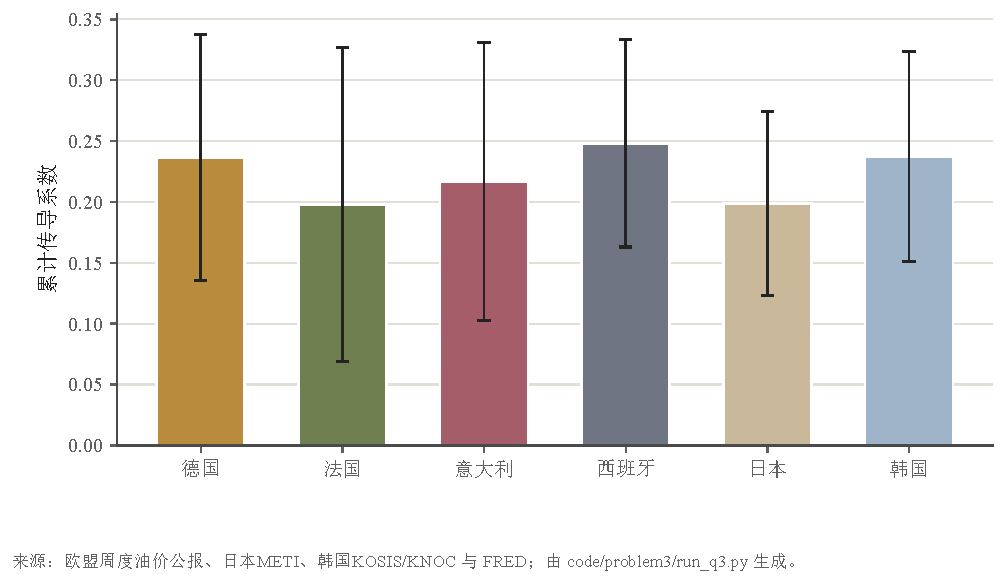
\includegraphics[width=0.91\textwidth]{../figures/q3_pass_through_6m.pdf}
  \caption{六国正式零售价格与中国调价指数代理的六个月传导率}
  \label{fig:q3-pass}
\end{figure}

\begin{table}[htbp]
  \centering
  \small
  \caption{六个月燃油传导率及数据角色}
  \label{tab:q3-pass}
  \begin{tabular}{lccccccc}
    \toprule
    国家 & 中国 & 德国 & 法国 & 意大利 & 西班牙 & 日本 & 韩国 \\
    \midrule
    传导率 & 0.373 & 0.237 & 0.198 & 0.217 & 0.248 & 0.199 & 0.237 \\
    数据角色 & 代理敏感性 & 正式 & 正式 & 正式 & 正式 & 正式 & 正式 \\
    \bottomrule
  \end{tabular}
\end{table}

六个正式对照国中位数为0.227。中国代理值0.373较高，但二者并非同类价格层，故不能据此判断
中国更优或更差。这个“不可比”结论本身是重要的数据审计结果。

\subsection{代理排名的临界误差与部分识别}

为了把“不可比”从定性提醒改成可检验边界，定义中国真实固定品类零售价格传导率与调价指数代理
之间的缩放关系

\begin{equation}
  \Pi_{\mathrm{CN,true}}=\kappa \Pi_{\mathrm{CN,proxy}}.
  \label{eq:q3-kappa}
\end{equation}

以六国中位数0.227和中国代理值0.373计算，临界缩放系数为
$\kappa^\ast=0.227/0.373=0.607$。这意味着：只有当真实固定品类零售价的六个月传导约低于
调价指数代理变化的61\%时，中国才可能落到六国中位数以下。长度为6个月的时间块bootstrap给出
均匀缩放情形下$\kappa^\ast$中位数0.590，95\%区间为$[0.436,0.834]$；前置折价与后置折价扰动
下区间分别为$[0.461,0.849]$和$[0.578,1.169]$。因此该计算只能量化代理误差需要多大，不能
把中国重新放回正式国别排名。

\begin{figure}[htbp]
  \centering
  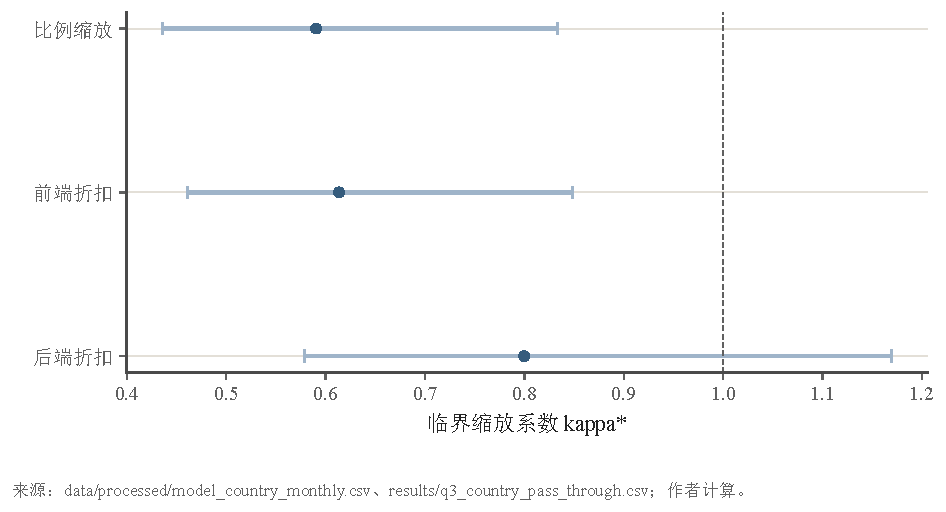
\includegraphics[width=0.72\textwidth]{../figures/paper_extension_q3_partial_identification.pdf}
  \caption{中国代理传导率进入正式排名所需的临界缩放系数}
  \label{fig:q3-partial-identification}
\end{figure}

\subsection{相对宏观响应与暂缓的机制回归}

对CPI和工业活动估计含国家固定效应和完整年月固定效应的面板局部投影：

\begin{equation}
  y_{i,t+h}-y_{i,t-1}=\alpha_{i,h}+\lambda_{t,h}
  +\delta_{i,h}(s_tI_i)+\Gamma_h^{\mathsf T}Z_{i,t-1}+u_{i,t+h}.
  \label{eq:panel-lp}
\end{equation}

中国是参照组，$\delta_{i,h}$只表示对照国相对中国的响应差，不能把中国绝对响应人为设为零。
对照国减中国的CPI相对响应点估计中位数为0.245个百分点，工业活动为2.433个百分点；但当前
程序没有形成联合国别--时间bootstrap区间，因此两项均判为“结论不充分”。价格监管、进口依赖、
石油强度和进口来源集中度年度表均为未经审计代理，四类连续缓冲交互回归全部执行失败关闭，不提供
系数、显著性或政策排序。三维核心韧性判据见表\ref{tab:q3-resilience}。

\begin{table}[htbp]
  \centering
  \small
  \caption{中国相对韧性的核心判据}
  \label{tab:q3-resilience}
  \begin{tabularx}{0.96\textwidth}{p{0.23\textwidth}Xp{0.22\textwidth}}
    \toprule
    维度 & 当前证据 & 判断 \\
    \midrule
    燃油价格 & 中国仅有调价指数代理，不能与六国固定品类零售价正式排名 & 条件代理 \\
    消费价格 & 对照国减中国点估计中位数0.245，缺联合差异区间 & 结论不充分 \\
    工业活动 & 对照国减中国点估计中位数2.433，缺联合差异区间 & 结论不充分 \\
    \midrule
    总体 & 任一核心维度均不足以形成稳健“更好”判断 & 结论不充分 \\
    \bottomrule
  \end{tabularx}
\end{table}

\subsection{关闭2026年临时调控的动态反事实}

依据《石油价格管理办法》\cite{ndrc2016}和2026公告核验，3月汽油机制应调2205元/吨、实调
1160元/吨，新增缺口1045元/吨；4月机制应调800元/吨、实调420元/吨，新增380元/吨，累计
缺口1425元/吨。令$P_t^{no}$和$P_t^{act}$分别为无临时调控与实际代理价格路径，输入模型的不是
静态价格水平差，而是逐月收益差

\begin{equation}
  \Delta f_t=100\left[\ln\frac{P_t^{no}}{P_{t-1}^{no}}
  -\ln\frac{P_t^{act}}{P_{t-1}^{act}}\right].
  \label{eq:fuel-return-gap}
\end{equation}

对$y\in\{PPI,CPI,IAV\}$，用0至6阶动态核和结果变量AR(1)递推：

\begin{equation}
  B_{y,t}=\sum_{\ell=0}^{6}\beta_{y,\ell}\Delta f_{t-\ell}
  +\phi_yB_{y,t-1}.
  \label{eq:policy-dynamic}
\end{equation}

三条方程使用同一组长度为6的循环时间块联合抽样，共接受2000组参数抽样，从而保留PPI、CPI和
IAV估计误差的同期相关。

\begin{figure}[htbp]
  \centering
  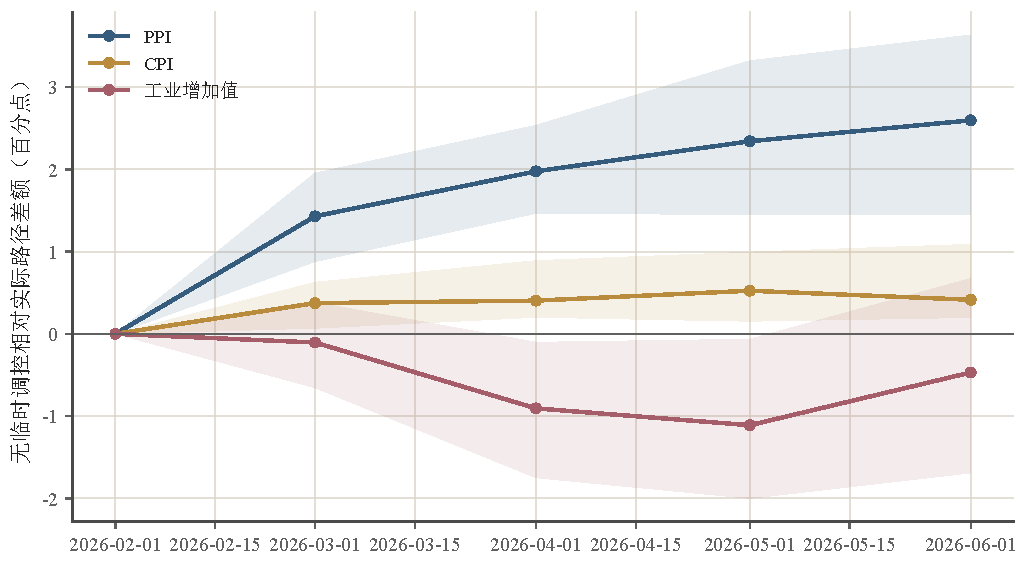
\includegraphics[width=0.91\textwidth]{../figures/q3_policy_macro_counterfactual.pdf}
  \caption{关闭临时调控后的动态宏观情景差额}
  \label{fig:q3-policy-macro}
\end{figure}

\begin{table}[htbp]
  \centering
  \small
  \caption{2026年6月无临时调控减实际路径的宏观差额}
  \label{tab:q3-policy}
  \begin{tabular}{lccc}
    \toprule
    变量 & 情景差额/百分点 & 95\%区间 & 情景证据 \\
    \midrule
    PPI & 2.596 & $[1.453,3.633]$ & 区间不跨零 \\
    CPI & 0.414 & $[0.199,1.088]$ & 区间不跨零 \\
    IAV & $-0.469$ & $[-1.690,0.672]$ & 结论不充分 \\
    \bottomrule
  \end{tabular}
\end{table}

结果说明，在维持动态核与局部环境不变的条件下，临时调控可能降低了2026年6月PPI和CPI压力；
IAV方向符合缓冲解释但区间跨零。该结论依赖调价指数代理，不能外推为全面福利改善，也不改变跨国
总体韧性“结论不充分”的判断。

\begin{table}[htbp]
  \centering
  \small
  \caption{政策工具、作用渠道与证据等级}
  \label{tab:q3-policy-evidence}
  \begin{tabularx}{0.98\textwidth}{p{0.18\textwidth}Xp{0.20\textwidth}p{0.20\textwidth}}
    \toprule
    政策工具 & 作用渠道 & 正文证据 & 证据边界 \\
    \midrule
    成品油价格监管 & 延缓原油成本向PPI和CPI传导，同时形成未调价缺口 & 2026年动态反事实；PPI、CPI区间不跨零 & 条件情景，不等于福利评估 \\
    进口来源多元化 & 降低单一区域供给中断暴露 & 机制解释与数据审计 & 连续HHI未审计，不估计交互系数 \\
    石油进口依赖度 & 决定国际价格冲击进入国内成本的暴露度 & 文献机制与国别描述 & 年度代理不足以支持月度因果结论 \\
    石油强度 & 决定单位产出的燃油和运输成本敏感性 & 文献机制与产业链解释 & 不恢复未审计缓冲回归 \\
    战略储备、汇率与财政措施 & 通过库存释放、汇率稳定和补贴减轻短期压力 & 作为边界条件讨论 & 缺连续、可比强度数据，不作量化排序 \\
    \bottomrule
  \end{tabularx}
\end{table}

\subsection{问题三小结}

正式零售价格、相对宏观响应和政策反事实属于三类不同证据。当前数据不能证明中国在三维韧性上
全面优于对照国；较强的结论只限于2026年条件情景中PPI与CPI的局部缓冲，同时必须显式记录
1425元/吨延期缺口及其后续消化责任。
